\documentclass{standalone}
\usepackage{tikz}
\usepackage{ctex,siunitx}
\setCJKmainfont{Noto Serif CJK SC}
\usepackage{tkz-euclide}
\usepackage{amsmath}
\usepackage{wasysym}
\usetikzlibrary{patterns, calc}
\usetikzlibrary {decorations.pathmorphing, decorations.pathreplacing, decorations.shapes,}
\begin{document}
\small
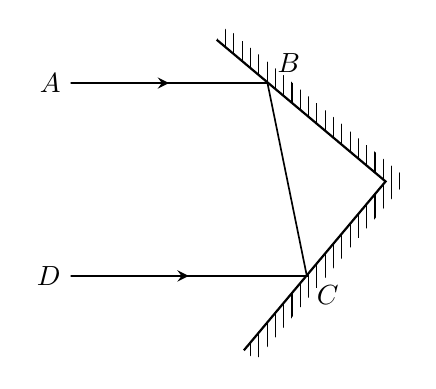
\begin{tikzpicture}[>=stealth,scale=1]
  \fill  [pattern=vertical lines, rotate=50] (-2.8,0)--(0,0)--(0,2.8)--(.2,2.8)--(.2,-.2)--(-2.8,-.2)--(-2.8,0);
  \draw [rotate=50,thick](-2.8,0)--(0,0)--(0,2.8);
  \draw[semithick] (-4,1.25)node[left]{$A$}--(-1.5,1.25)node[above right]{$B$}--(-1,-1.2)node[below right]{$C$}--(-4,-1.2)node[left]{$D$}  ;
  \draw[thick, ->] (-4,1.25)--(-5.5/2,1.25);
  \draw[thick, <-] (-2.5,-1.2)--(-4,-1.2);
\end{tikzpicture}
\end{document}